% Бүлэг 2

\chapter{Прокси дахин шифрлэлтэд суурилсан файл хуваалцах систем} % Зарим нэг зөвлөмж
\label{Chapter2} % Энэ бүлэг рүү ишлэл хийх бол \ref{Chapter2} командыг ашигла 
\pagecolor{white}

%-------------------------------------------------------------------------------
%	SECTION 1
%-------------------------------------------------------------------------------
\section{Прокси дахин шифрлэлт}
Прокси дахин шифрлэлт нь нийтийн түлхүүрээр шифрлсэн өгөгдөлийг дахин ширфлэж өөр хувийн түлхүүрээр тайлах боломжийг олгодог.

Мамбо болон Окамото шифрийг тайлан дараа нь шифрлэх уламжлалт аргыг сайжруулах зорилгоор анх гаргаж ирсэн.

1998 онд Blaze, Bleumer, Strauss (BBS) нар "atomic proxy cryptography" гэсэн ойлголтыг санал болгосон бөгөөд үүнд хагас итгэмжлэгдсэн прокси нь үндсэн энгийн текстийг харалгүйгээр Алисын шифрийг Бобын шифр текст болгон хувиргадаг. El Gamel дээр суурилсан схем ба прокси буюу гуравдагч талийн тусламжтайгаар шифрийг дамжуулах зорилготой. 

\textbf{Үндсэн хоёр төрөлтэй.}
\begin{itemize}
    \item Нэг чиглэлт (Unidirectional PRE)
    \item Хоёр чиглэлт (Bidirectional PRE)
\end{itemize}

Нэг чиглэлт PRE (KE, RG, E, R, D) хэсгүүдээс тогтоно.

\begin{enumerate}
    \item Алис, Боб болон Чарли хувийн болон нийтийн түлхүүрийг үүсгэнэ. (KE)
    \item Алис Боб-д зориулж өгөгдлөө шифрлэж серверт байршуулна.
    \item Боб Алис-ын өгөгдлийг Чарли-тай хуваацлахын тулд RE(pkB,skB,pkC,skC∗) шифрлэж серверт байршуулна. Чарлигийн хувийн заавал шаардахгүй үүсгэж болно.
    \item Боб RE-г ашиглаж үүсэгсэн түлхүүрийг серверт явуулж Алисын файлыг дахин шифрлэж Чарли тайлах боломжтой болно.
\end{enumerate}

\begin{figure}[ht]
\centering
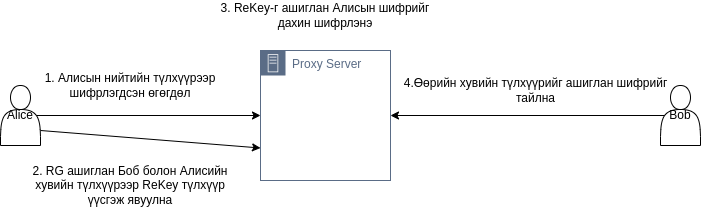
\includegraphics[scale=0.5]{Figures/PRE.drawio.png}
\caption[Proxy Re-encryption scheme]{Proxy Re-encryption scheme}
\label{fig:PRE_Scheme}
\end{figure}

Давуу талууд:
\begin{itemize}
    \item Нууцлалыг сайжруулна: PRE нь оролцогч талуудын хувийн мэдээллийг задруулахгүйгээр өгөгдлийг хуваалцахыг зөвшөөрснөөр нууцлалыг сайжруулахад тусална. Энэ нь талууд нууцаар эсвэл хувийн нууц мэдээллийг задруулахгүйгээр мэдээллээ хуваалцахыг хүссэн тохиолдолд хэрэг болно.
    \item Нарийн төвөгтэй байдлыг багасгасан: PRE нь итгэмжлэгдсэн гуравдагч этгээдэд шифрлэлт болон шифрийг тайлах үйл явцыг удирдах боломжийг олгосноор шифрлэлт болон түлхүүрийн удирдлагын нарийн төвөгтэй байдлыг багасгахад тусална. Энэ нь ялангуяа олон талын оролцоотой, гол менежмент нь төвөгтэй, удирдахад хэцүү болж болзошгүй тохиолдолд хэрэг болно.
\end{itemize}

Сул талууд:
\begin{itemize}
    \item Проксид итгэх: PRE нь дахин шифрлэлтийг гүйцэтгхэд гуравдагч талын прокси дээр тулгуурладаг ба схемийн аюулгүй байдал нь прокси талаас хамаарна.
    \item Хязгаарлагдмал өргөтгөх чадвар: PRE нь өргөтгөх чадварын хувьд хязгаарлагдмал байж болно. Учир нь хэрэглэчдийн тоо нэмэгдэхийн хэрээр олон талыг дэмжихэд шаардлагатай дахин шифрлэлтийн түлхүүрүүдийн тоо хурдацтай өсөх болно. Энэ нь гол менежментийг төвөгтэй болгож, удирдахад хэцүү болгодог.
    \item Potential for replay attacks: PRE нь халдагч хариуг зогсоож хандах эрхийг өөрт ашигтай солих боломжтой. 
    \item Хүчингүй болгоход хүндрэлтэй байдал: PRE дахь өгөгдөлд хандах эрхийг цуцлах нь ялангуяа олон тал оролцсон тохиолдолд хэцүү байж болно. Хэрэв аль нэг талын дахин шифрлэлтийн түлхүүр алдагдсан бол бусад талуудын мэдээлэлд хандах эрхэд нөлөөлөхгүйгээр өгөгдөлд хандах эрхийг цуцлах нь хэцүү байж болно.
    \item Хязгаарлагдмал хэрэглээ: PRE нь харьцангуй шинэ бөгөөд шинээр гарч ирж буй технологи хэвээр байгаа бөгөөд илүү уламжлалт шифрлэлтийн схемүүдтэй харьцуулахад хэрэглээ нь хязгаарлагдмал байдаг. Энэ нь технологийг хэрэгжүүлэх, удирдах туршлагатай мэргэжилтнүүд бага байдаг.
\end{itemize}

%-------------------------------------------------------------------------------
%	SECTION 2
%-------------------------------------------------------------------------------
\section{Хөгжүүлэх технологи, хэл сонгох}

Прокси дахин шифрлэлт файл хуваалцах системийг хөгжүүлэхэд ашиглах технологийн судалаа хийсэн.
Систем хоёр хэсгээс тогтох ба. API сервер болон хэрлэгч талын программ. Пайтон маш олон нэмэлт бичиглэл хялбар олон давуу талтай тул пайтон хэлийг сонгосон. Үүнд:
\begin{itemize}
    \item Flask
    
    Пайтон хэл дээр бичсэн веб хөгжүүлэхэд зориулагдсан фреймворк юм. Хөнгөхөн олон сан шаардахгүй. Сурахад хялбар өөрийн хүссэн загвараар загварчилж хийх боломжтой. RESTFul API гаргахад хялбар. Хэрэгтэй гэвэл нэмэлт сан ORM зэрэг өөр сангууд суулгаж хамт ашиглах боломжтой.
    \item Tkinter
    
    Хэрэглэгчийн интерфейс (GUI) үүсгэхэд ашигладаг Python номын сан юм. Tcl/TK GUI дээр суурилсан. Линукс виндовс зэрэг олон үйлдлийн системийг дэмждэг. Нэмэлт сангуудтай ажиллах боломжтой.
    \item pyUmbral
    
    Прокси дахин шифрлэлтийг файтон дээр хэрэгжүүлсэн пайтоны сан юм. OpenSSL болон Cryptography.io ашиглсан.
    \item Google Cloud Platform
    
    Хийсэн API сервер deploy хийж байршуулна. Google Cloud нь маш олон давуу талтай ба үнэгүй туршиж үзэх 300 долларын эрхтэй тул сонгосон.
\end{itemize}

%-------------------------------------------------------------------------------
%	SECTION 3
%-------------------------------------------------------------------------------
\section{Хөгжүүлэлтийн орчин бэлдэх}

Пайтон хэл нь орчин бүрдүүлхэд хялбар ба виртуал орчин үүсгэж хэрэгтэй сангуудийг татаж суулгах боломжтой. Бүх линукс тархацад пайтон хэл нь сууцан байдаг тул хэрэгтэй сангуудийг татаж суулгахад л хангалтай.

Прокси дахин шифрлэлт сан пайтон дээр сан бичих гэж оролдсон. JHU-MTI Прокси дахин шифрэлэлтын сан нь C/C++ хэл дээр бичигдсэн байсан. Пайтон хэлний setuptools болон C хэлний "python.h" санг ашиглан пайтоны сан бичих гэж оролдож үзсэн. JHU-MTI сан нь MIRCL санг ашигладаг.
\textbf{Ерөнхий бүтэц}
\dirtree{%
.1 ..
.2 example.
.3 example.py.
.2 external.
.3 miracl.
.3 proxylib.
.2 LICENSE.
.2 README.md.
.2 setup.py.
.2 src.
.3 pypre.cpp.
.2 userguide.pdf.
}

% эхлүүлсэн болов ч цагтаа амжихгүй болсон тул pyUmbral гэдэг санг ашиглсан. 

%-------------------------------------------------------------------------------
%	SECTION 4
%-------------------------------------------------------------------------------
\section{Бүлгийн дүгнэлт}
Прокси дахин шифрлэлт судлаж системийг хөгжүүлэлтэнд шаардлагатай технологиуд сангуудыг судлаж хөгжүүлэлт хийж эхэлсэн.